\documentclass[12pt, oneside]{article} 
\usepackage{booktabs}
\usepackage{geometry}              	
\usepackage{adjustbox}
\usepackage{pdfpages}  		
\usepackage{graphicx}
\usepackage{caption}						
\usepackage{amssymb}
\usepackage{amsmath}
\usepackage{pdfpages} 
\usepackage{longtable}
\usepackage{subfig}
\usepackage{url}
\usepackage{comment}
\usepackage{microtype}
%\usepackage{subcaption}
\usepackage{graphicx}  % remove 'demo' option for your real document

\usepackage{fancyvrb}
\usepackage{hyperref}
\hypersetup{colorlinks,linkcolor={blue},urlcolor={black},citecolor={blue}}  
\usepackage{titlesec}
\usepackage{fancyhdr}
\usepackage{blindtext}
\usepackage{graphicx}
\usepackage{longtable}
\usepackage{booktabs}
\usepackage{multirow}
%\usepackage[dvipsnames]{xcolor}
\usepackage{pdflscape}
\usepackage{subfig}
\setcounter{tocdepth}{6}
\setcounter{secnumdepth}{6}
\titleformat{\paragraph}
{\normalfont\normalsize\bfseries}{\theparagraph}{1em}{}

 \setlength{\headheight}{14.5pt}
\lhead{}
 
\usepackage[english]{babel}
\usepackage[utf8]{inputenc}

\geometry{left=2.0cm,right=2.0cm,top=2.0cm,bottom=2.0cm}
%using the euro symbol
\usepackage[utf8]{inputenc}
\usepackage{marvosym}
\DeclareUnicodeCharacter{20AC}{\EUR{}}
%\usepackage[dvipsnames]{xcolor}
\usepackage{array,tabularx,calc}
%to allow use of < and >
\usepackage[T1]{fontenc}
%references
\usepackage{csquotes}
%\usepackage[style=nature]{biblatex}
%\addbibresource{references.bib}
\newlength{\conditionwd}
\newenvironment{conditions}[1][where:]
  {%
   #1\tabularx{\textwidth-\widthof{#1}}[t]{
     >{$}l<{$} @{${}={}$} X@{}
   }%
  }
  {\endtabularx\\[\belowdisplayskip]}

\usepackage{array,tabularx}

\newcommand{\HRule}[1]{\rule{\linewidth}{#1}} 	% Horizontal rule

\makeatletter							% Title
\def\printtitle{%						
    {\centering \@title\par}}
\makeatother
									

\makeatletter							% Author
\def\printauthor{%					
    {\centering \large \@author}}				
\makeatother	

\usepackage{mathtools} 

\usepackage[font=small,labelfont=bf]{caption}

\begin{document}

%\renewcommand{\labelenumii}{\Arabic{enumii}}





\begin{titlepage}
    \centering 
	\scshape
	\vspace*{2\baselineskip}
	\rule{\textwidth}{1.6pt}\vspace*{-\baselineskip}\vspace*{2pt} 
	\rule{\textwidth}{0.4pt} 
	\vspace{0.75\baselineskip} 
	{\Huge EOSC595 \\ Directed Study in Polar Climate} \\
	\vspace{0.1in}
		{\Large Literature Review} \\
		\vspace{0.1in}
		{\Large Ruth Moore} \\
	\vspace{0.75\baselineskip} 
	\rule{\textwidth}{0.4pt}\vspace*{-\baselineskip}\vspace*{2pt} 
		\rule{\textwidth}{1.6pt}
	\vspace*{2\baselineskip} 

\Huge{Understanding the Arctic atmospheric hydrological cycle and how it's changing}
\vspace{0.1in}	

\begin{figure}[hbtp]
\centering

\includegraphics[width=0.5\textwidth]{../ubc-logo-png-transparent.png}
\end{figure}
{\Large Spring 2023} \\
	{\large University of British Columbia} 
\end{titlepage}
\pagestyle{fancy}


{
  \hypersetup{linkcolor=black}
  \tableofcontents
}


\thispagestyle{empty}
\clearpage
\setcounter{page}{1}


\pagebreak





%\begin{center}
%	\hrule
	%\vspace{.4cm}
	%{\textbf { \large EOSC 595: Directed study, Arctic Climate change \\ An updated review on Arctic warming and it's implications on the hydrological cycle}}
%\end{center}
%{\textbf{Name:}\ Ruth Moore \hspace{\fill} }\textbf{Date:} March 3rd 2022   \\
	%\hrule

%\hfill
%\hfill
% \hfill
%\hfill

\section{Introduction}
\subsection{The changing hydrological cycle of the Arctic}
In recent years many papers have been written on the state of knowledge of Arctic warming and amplification\cite{davy2018arctic, previdi2021arctic, vihma2016atmospheric, serreze2011processes} as well as the changing hydrological cycle. As we better understand concepts such as cloud microphysics\cite{pithan2014mixed} and water vapour transport\cite{gimeno2019atmospheric}, our understanding of the changing weather of the region improves. Recent updates such as the Arctic Report Card 2022\cite{druckenmiller2022arctic} give updated information on the changes seen by the region.


Considerable progress has been made in the understanding of polar amplification in the Arctic over the last decades, the phenomenon in which the poles are warming more quickly than the rest of the world. In recent years we have begun to understand why these changes are occurring, and increasingly the cause for this warming has been attributed to an increase in precipitation and humidity \cite{dou2022more}. This review will focus specifically on how the climate of the Arctic region is causing changes to the atmospheric hydrological cycle, changes which rely heavily on local geography and weather. 


This review is split up into three major sections. The first looks at important background information required understand when discussing change in the Arctic region, defining the Arctic region, section \ref{arctic}, physical mechanisms, section \ref{mechanisms} and defining Arctic change section, \ref{arctic change}. The second looks to understand the atmospheric hydrological cycle, section \ref{the cycle}. The third looks at how the cycle is changing section \ref{change}, which is split up into local changes, section \ref{local} and remote changes, section \ref{remote}. Finally, a discussion is given on gaps in knowledge, section \ref{gaps}. 

%define all of the variables which are seeing change and combine them together on one figure



\subsection{The importance of the Arctic within the global climate system}
The Arctic is closely linked to the rest of the global climate system. The loss of ice in the Arctic has a larger impact on global sea level rise than melting in Antarctica\cite{AMAP}. The melting of sea ice and the cryosphere reduce the overall albedo of Earth which further increases heat absorption from the sun.

The melting of sea ice in the North Atlantic is causing the Atlantic Meridional Overturning Circulation (AMOC) to slow down, which will result in Europe in the future having harsher, colder and wetter winters \cite{jackson2015global}. 

Changing Arctic ecosystems can also induce changes on global scales. The increase of wildfires results in an increase of carbon emissions to the atmosphere. The greening of the tundra is resulting in changes to migration patterns. The melting sea ice and permafrost is also resulting in new shipping routes being opened and proposed and increased opportunity for mining\cite{AMAP}. All of these environmental changes are also having direct impacts on local livelihoods on the people of the Arctic.  

Some work has shown that the dynamics of the Arctic also effect mid-latitude weather through changes in storm tracks, the jet stream, and planetary waves\cite{cohen2014recent}. These changes in the mid-latitudes are resulting in more extremes like droughts.n

Overall, the Arctic is an important factor in the dynamics of the global climate system, and therefore understanding the hydrological cycle within the region, and how it is changing is crucial for developing a more thorough understanding of climate dynamics and change as a whole.

\section{The Arctic as a region}\label{arctic}
\subsection{How we define the Arctic}
The Arctic, or North Pole is the most northerly region on Earth. It is generally geographically defined as the region north of 66.5°, which is the region above the Arctic circle. Some definitions of the Arctic are based on the region north of the 10 °C isotherm in July, which also corresponds to the tree line, and the region of the Arctic is which is not above 10 °C even in summer\cite{boulder}.  

However, when it comes to analysis within the Arctic region, there is no agreed upon definition for where the Arctic begins. For simplicity, most papers refer to the Arctic region as being anywhere from 60°N where some define it as 70°N\cite{Ghatak2013, serreze2012recent}. These discrepancies in latitudinal definition can often help to explain how different papers will give different or conflicting results for similar analysis.% (give evidence)
\subsection{The regions of the Arctic}
The Arctic can generally be split up into the regions of the Arctic Ocean, the land from the continents of North America and Eurasia, and the sea ice which changes extent with each winter and summer freeze thaw cycle. 

\subsection{The influence of local geography on hydrological cycle changes}
The changes in sea ice extent and thickness, transport of moisture and heat, humidity and precipitation all rely heavily on local geography and weather. Therefore, in this review and in other similar literature, we split the hydrological changes which are occurring into local and remote. Local changes are generally directly linked to ice melt and local warming, section \ref{local}, which remote changes are due to dynamical influences of storms and other methods of moisture transport, section \ref{remote}.




\section{Important physical mechanisms}\label{mechanisms}

\subsection{Defining climate forcings, feedbacks and mechanisms}
\subsubsection{Climate forcings}
Climate forcings are physical processes which alter the climate system. They are external factors which can be natural (such as volcanic effects) or anthropogenic (such as greenhouse gases). 

\subsubsection{Feedbacks}
Climate feedbacks are processes which alter the climate system. Positive feedbacks result in an increase in a phenomenon when the forcing is increased, and negative feedbacks result in a decrease in the phenomenon when the forcing is increased. 

Feedbacks can be described as the response of the climate system to a forcing. Feedbacks can also be internal. 

\subsubsection{Mechanisms}
Mechanisms are physical processes which are used to explain how changes occur within the climate system. An example of a climate mechanism is the formation of deep water in the North Atlantic which drives the AMOC.

\subsection{Humidity}\label{humidity}

Humidity is the concentration of water vapour present in the air. It depends on the temperature and pressure of the system of interest, with three measurements used; relative, absolute and specific humidity. 

In the Arctic humidity changes can occur both due to local sea ice losses, section \ref{local} and the transport of moisture from other regions' section \ref{remote}. 


\subsubsection{Absolute humidity}
Absolute humidity ($\rho_v$) is the mass of water vapour per unit volume of air, and does not take temperature into consideration\cite[p.~91]{stull2015practical}.

\begin{equation}
    \rho_v = \frac{m_{vapor}}{Volume}
\end{equation}
here $m_{vapor}$ is the mass of water vapour and $Volume$ is the volume of air and water vapour mixture. These quantities are easy to measure and give the actual concentration of vapour in the air. 



\subsubsection{Specific humidity}
Specific humidity ($q$) is the ratio of water vapour mass to total moist air parcel mass. It is approximately equal to the mixing ration which is the ration of mass of water vapour in an air parcel to the mass of dry air for the same sized parcel \cite[p.~91]{stull2015practical}. 
\begin{equation}
    q = \frac{m_{vapour}}{m_{air}}
\end{equation}
Here $m_air$ is the mass of air. Specific humidity is not affected by heating, cooling and pressure changes. 


\subsubsection{Relative humidity}
Relative humidity (RH) is the ratio of the partial pressure of water vapour in a mixture (i.e. the air) to the equilibrium vapor pressure of water over a flat surface of pure water. This measurement is the ratio of how much water vapour is in the air versus how much it could have \cite[p.~92]{stull2015practical}.
\begin{equation}
    RH = \frac{e}{e_s}
\end{equation}

Where e is the vapour pressure, and $e_s$ is the saturated vapour pressure. Relative humidity regulates the maximum possible evaporation into air and is useful when discussing humidity changes as it is related to the temperature of the air. Since warmer air has more water vapour than cooler air, it will have a higher relative humidity when the air is cooler and a lower relative humidity when the air is warmer, even though the specific and absolute humidity in these cases is the same. 




\subsection{The Clausius-Clapeyron relation}\label{cc}
The capacity of air to hold moisture increases exponentially with air temperature according to the Clausius-Clapeyron equation. Saturated water pressure P and temperature T are related as follows (temperature in Kelvin) \cite[p.~88]{stull2015practical};

\begin{equation}
    e \approx e_0  \cdot exp  \left ( \frac{L}{R_v} \left (  \frac{1}{T_0} - \frac{1}{T}  \right ) \right )
\end{equation}

Where $R_v$ is the water-vapor gas constant, 461 $J \cdot K ^{-1} \cdot kg ^ {-1}$, $T_0$ = 273.15 K, $e_0$ = 0.6113 kPa and L is the latent heat parameter. 

This equation allows and estimate of vapour pressure at different temperatures and visa-versa, which simplifies to an increase of water retention by around $7\% / ^{\circ} C $. This would lead to a strengthening of the global evaporation (E) minus precipitation (P) pattern with overall global surface temperature increases\cite{held2006robust}. Experimental results differ from this estimation, and it has been found to have a value closer to $3.0 \pm 1.6 \% / ^{\circ} C $ from 1950 to 2010, with climate models showing an increase of $4.3 \pm 2.0 \% / ^{\circ} C $ under greenhouse gas emission scenarios\cite{Skliris2016}. 






\section{Defining Arctic Change}\label{arctic change}
As discussed, the Arctic is changing, and at a rate which is quicker than other parts of the globe. When discussing the changing climate and temperatures of the Arctic five terms are important to define; Arctic warming, polar and Arctic amplification, anthropogenic forcing and internal variability. 



\subsection{Arctic warming}
Arctic warming is the general increase of temperature in the Arctic region. This is a result of greenhouse gas emissions, increases in $CO_2$ in the atmosphere. Arctic warming is as a result of anthropogenic influences on the global climate system. 

Arctic climate change is mainly characterized by a warmer and wetter atmosphere due to the overall global increase in temperature. 

\subsection{Polar Amplification}\label{polar_amplification}
Polar amplification is the phenomenon in which any change in net radiation balance on Earth produces larger temperature changes in the poles than on the rest of the planet. This is a `natural' feature of our global climate which is as a result of water-vapour radiative feedbacks, meridional moisture and heat transport, and snow and ice albedo feedbacks. Polar amplification can be seen in the paleo record\cite{miller2010arctic}, where Arctic temperature changes are seen to consistently be about 3-4 times greater than the rest of the Northern Hemisphere, Arctic temperature anomalies are a normal feature of the global climate.


However, this `natural' feature is currently being heavily influenced by anthropogenic forcing. Recently with severe increases in global temperature, rate of polar amplification has increased. The severe loss of sea ice and snow cover, the confinement of warming to the near surface in the polar atmosphere and the increases in poleward atmospheric and oceanic heat transport have caused the polar regions to warm considerably. These processes are all combined effects which differ between the hemispheres.

There has been a considerable loss in sea ice extent since 1979, with a yearly decrease in sea ice expected to continue with the increase in $CO_2$ in the atmosphere. With warming temperatures ice has less time to form which makes it thinner and causing it to melt earlier, further amplifying the warming. 

%There has been an increase in atmospheric and ocean heat transport to the poles due to changes in the transport of latent energy (moisture) and dry static energy (the sum of sensible and potential energy) by atmospheric circulations. This process can be described using an Earth System Model, where eddies dominate heat transfer from the mid-latitudes to the poles. As the mid-latitudes warm this increases the difference in moisture between the poles and the mid-latitudes causing an increase in poleward latent heat energy transport. 

%This episodic increase in latent heat transport into the poles results in an enhancement of the surface down welling radiation, which drives sea ice losses on sub-seasonal timescales. 


\subsubsection{Arctic Amplification}

Polar amplification effects the Northern Hemisphere more than the Southern Hemisphere. This is due to the larger surface heat uptake in the Southern Ocean and the asymmetry in radiative feedbacks in the poles. Therefore, the changes described in section \ref{polar_amplification} occur more severely and intensely in the Arctic compared to Antarctica, this is known as Arctic amplification\cite{england2021recent}. 

The increase in Arctic annual mean surface temperature (land and ocean) between 1971 and 2019 was three times higher than the increase in the global average during the same period\cite{AMAP}.

There is a seasonality to the phenomenon in which there is a peak of sea ice losses in early winter and increases in heat fluxes from the ocean to the atmosphere resulting in strong near surface warming. This results in Arctic amplification being stronger during the winter months, with winter warming being almost four times stronger than summer warming\cite{bintanja2013changing}. 


\subsection{Anthropogenic forcing}
Anthropogenic forcing refers to any human induced influence on the climate system. A large proportion of recent changes in the Arctic can be attributed to influences from anthropogenic forcings, such as increased greenhouse gases and the overall global temperature rise since pre-industrial times. Anthropogenic forcings are the primary drivers of human induced climate change and are resulting in recent Arctic changes occurring at an unprecedented rate. 


\subsection{Internal variability}
Some recent changes in the Arctic climate system can also be attributed to internal variability. The internal variability of the Arctic climate system is still relatively unknown, but some studies have shown, using ensembles from models, that internal variability can play a large role in Arctic climate. An example of this is\cite{ding2019fingerprints} which shows that up to 50\% of recent sea ice changes could be attributed to internal variability. 


\section{The Arctic atmospheric hydrological cycle}\label{the cycle}
%An introduction to the atmospheric hydrological cycle of the Arctic

%Include the sketch of the hydrological cycle explaining the basic mechanisms

%Introduce the mechanisms which will be talked about - do not repeat from introduction

%\subsection{Hydrological cycle}
%{\color{blue}- Why the moisture component is very important 
%- Sources of moisture and possible changes to this }
%\subsubsection{Phenomenon which effect humidity}
%{\color{blue}-  how the circulation of wind in the Arctic effects humidity 
%- sea ice 
%- evapotranspiration }

\subsection{The hydrological cycle}
The hydrological cycle describes the sum total of all processes in which water moves from the land to the ocean surface to the atmosphere and back to the land/ocean in the form of precipitation\cite{CHAKRAVARTY2019203}. 

The amount of moisture in the Arctic is determined by the rates of local evaporation and moisture transport from lower latitudes, see fig.\ref{fig:hydro_cycle}. 


As described in section \ref{cc} an increase in global temperatures increases the overall amount of moisture in the air. Moisture content in the Arctic is closely linked to increases in moisture in the mid-latitudes due to processes of poleward moisture and heat transport, as described in section \ref{polar_amplification}.

Terrestrial, marine and freshwater ecosystems are strongly coupled with the cryosphere and atmosphere to form the Arctic hydrological cycle, as shown in fig.\ref{fig:hydro_cycle}.  


\begin{figure}[h!]
\centering
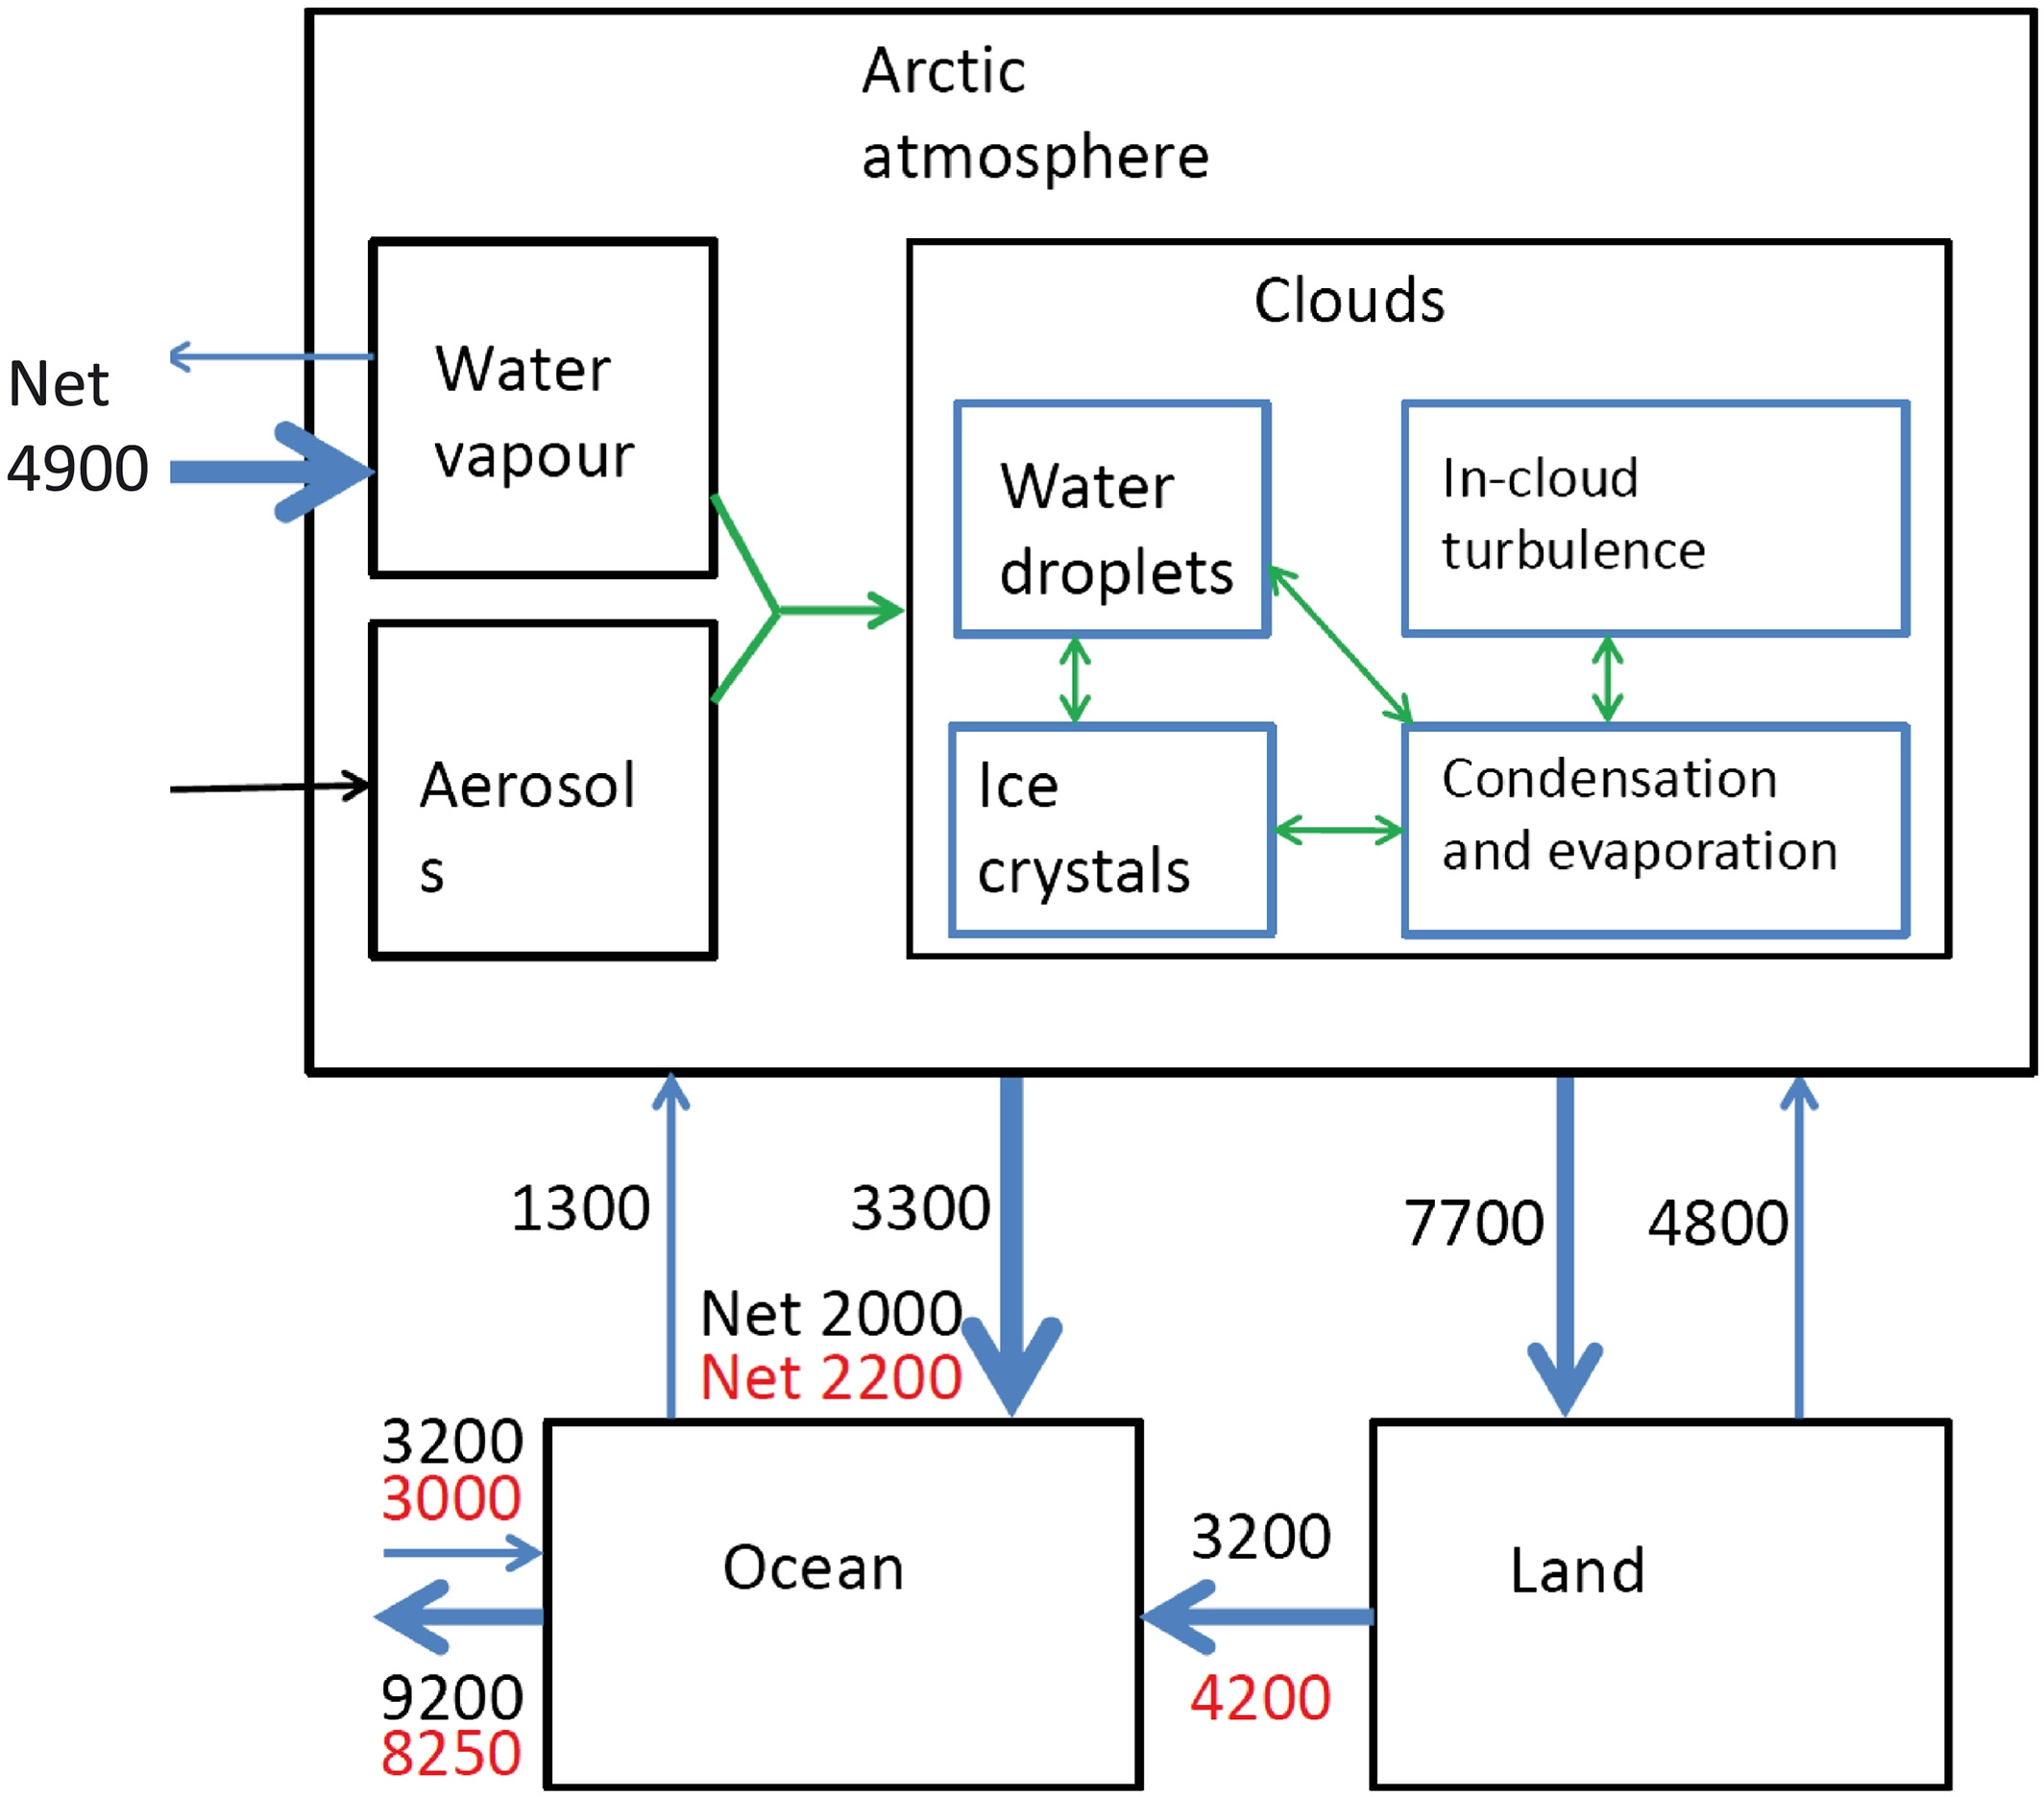
\includegraphics[width=0.7\textwidth]{hydological_cycle.png}
\caption{This schematic shows the main freshwater components and processes in the Arctic hydrological cycle\cite{vihma2016atmospheric}. The numbers in black show the main freshwater transports in $km^3/yr$ based on\cite{serreze2006large} for 1979-2010, with the numbers in red show the estimates for 2000-2010 from\cite{haine2015arctic}. }\label{fig:hydro_cycle}
\end{figure}

\subsection{Temperature influences}\label{temp}
Temperature increases drive ice losses and overall increase in the amount of moisture in the region. The increased temperature results in changes in humidity as the warmer air can hold more moisture section \ref{cc}.

The uneven heating of the globe drives atmospheric heat transport\cite{Goosse2018}. Within the Arctic, temperature changes are not evenly distributed, with local variability between land and ocean being high due to heat capacity differences\cite{dufour2016atmospheric}, especially in the winter, when the ocean is warmer than the frozen land. 



\subsection{Arctic atmospheric moisture}

In the polar regions the atmospheric component of the hydrological cycle is composed of a moisture flux, where precipitation (P) and evaporation (E) converge to give net positive precipitation (P-E). Remote based condensation of transported atmospheric moisture and local recycling are the two main factors in Arctic precipitation. The balance of P-E is generally seen an input of freshwater from the atmosphere to the ocean\cite{oshima2017atmospheric}. The seasonal cycles of P-E over the regions are governed by cyclone cycles where interannual variations are determines by the Arctic Oscillation. 


Atmospheric moisture is composed of water vapour which is the source of cloud and fog formation. This affects radiative transfer, evaporation and condensation, where relative humidity controls cloud formation. During cloud formation, the amount of moisture at where saturation is reached depends on the vertical temperature profiles and specific humidity of the cloud. As the volume of unsaturated air cools, it's relative humidity increases since the ability for air to hold vapour decreases with temperature. The air temperature inversion generally occurs between 1-1.5 km, but this has strong seasonal and spatial variation. 

Changes in specific humidity effect long wave and shortwave radiative transfer in the atmosphere, where humid air emits more long wave radiation than dry air due to its humidity and temperature. 

%Water vapour in the Arctic has a residence time of around a week, compared with a decade for freshwater in the Arctic Ocean. 

The spatial and temporal distributions of water vapour are related to air temperature distributions. As explained in section \ref{cc} the moisture holding capacity of air increases exponentially with air temperature, and therefore total vertically integrated water vapour (TWV) decreases with increase in longitude, from summer to winter and is higher over the open ocean (which is warmer than the cryosphere). As a result clouds are more common over the open ocean than they are over icy regions, and are also sparse over the continents. The amount of cloud cover reaches a maximum in the mid-latitude Arctic regions in the late summer, and a minimum during the late winter. 

%add more detail here https://agupubs.onlinelibrary.wiley.com/doi/10.1002/2015JG003132


Most of the moisture in the Arctic during the summer is from the land (56\%) as opposed to remote sources\cite{harrington2021terrestrial}, with 47\% of that water vapour coming from Eurasia as opposed to North America and Greenland.



\subsubsection{Cloud cover}
Cloud cover is difficult to determine in the Arctic due to temporal and spatial limitations, with data indicating that the Arctic has an annual cycle of cloudiness ranging from 40-70\% in winter to 80-95\% in summer \cite{vihma2016atmospheric}. Low clouds and fog dominate and predominantly have a warming effect on the surface, especially over the ice covered part of the Arctic Ocean. Cloudy conditions are often related to a warmer free troposphere, as cloudy episodes are typically associated with advection from lower latitudes. 


\subsubsection{Precipitation}
Arctic precipitation generally falls as snow or rain, with the seasonal cycle of drier winters and wetter summers lagging behind temperature by about one month. This value varies between regions. For most regions of the Canadian Arctic, precipitation peaks in August, this is after all the ice has melted following the summer period, so there is the maximum amount of water vapour avaialble\cite{serreze2022characteristics}. Generally the Canadian Arctic is drier than the Eurasian Arctic due there being less of an influence from the Atlantic sector. 


In winter the spatial distributions of precipitation and evaporation are dominated by the difference between large values over the open seas and low values over snow/ice-covered sea and land areas. In summer, both precipitation and evaporation occur over Arctic land areas, except Greenland, exceeding the values over sea areas north of 70$^{\circ}$N. This evaporation is comparable to those at lower latitudes \cite{vihma2016atmospheric}. 

Precipitation and evaporation/evapotranspiration affect the ocean and terrestrial freshwater budgets, the surface albedo and energy budget, and the mass balance of ice sheets, glaciers, and sea ice. 

\subsubsection{The influence of the cryosphere on atmospheric moisture}
Of the components which constitute the Arctic environment, the cryosphere is the most sensitive to the effects of the changing climate\cite{rinke2019trends}. The cryosphere, which is the ice component of the Earth's surface is closely linked with terrestrial and freshwater ecosystems, making it a crucial component within the Arctic system.

The changing cryosphere effects the overall hydrological cycle within the Arctic, contributing to the warmer and wetter conditions which have been seen in recent years. The cryosphere amplifies climate change through snow, ice and permafrost feedbacks. 

\paragraph{Sea ice}
Sea ice amount has a natural fluctuation within the Arctic climate system throughout the year, with coverage between 5 and 6 million $km^2$ at the end of the summer to 14 million $km^2$ at the end of winter. 

Sea ice extent and thickness has a large influence on the atmospheric hydrological cycle. The melting of sea ice is an example of a positive-feedback, where increased temperatures cause melting, which reduce albedo, which result in more heat uptake, and the cycle amplifies. In some cases, this melting results in low-lying clouds which have an albedo similar to ice and therefore the feedback is more muted. This increased melting is resulting in there being more available moisture in the air, and thus the humidity of the Arctic increasing. The increase in the amount of open water results in more surface area for evaporation and local moisture recycling. 

 Due to a large amount of evaporation from leads and polynyas, the near-surface air humidity over Arctic sea ice is generally close to saturation concerning the ice phase and therefore sublimation is weak\cite{andreas2002near}. 
 
 Leads are large fractures within an expanse of sea ice, where a linear area of open water is present, and often used for transport. They can vary in width from meters to hundreds of meters. Polynyas are areas of open water surrounded by sea ice. Both of which contribute to the amount of available moisture for evaporation.



\paragraph{Snow cover}
In the Arctic, snow can account for up to 80\% of total precipitation, with most net precipitation being stored as snow. Snow extent and fall is crucial to the hydrological cycle, where its albedo affects surface radiation balances and water budgets and the habitat of land and water organisms. Snow is an insulator affecting the thermal balances of the ground and permafrost distribution. 

Generally, in the Arctic region as a whole, snow mass peaks in early April with there being large interannual variability\cite{dufour2016atmospheric}. 

\paragraph{Permafrost}\label{permafrost}

The frozen component of the ground, such as rock and ice which remains permanently frozen is known as permafrost. Permafrost is composed of an upper layer which thaws during the summer and freezes again during the autumn/winter, which is known as the active layer. Permafrost covers approximately 25\% of and in the Northern Hemisphere and contains twice as much carbon as the atmosphere \cite{permafrost}. 

Frozen ground plays a very important role in the hydrological cycle due to its influence on runoff, groundwater storage, purity and flow and overall influences on water filtration. When active-layers thicken this can lead to  increased filtration, larger amounts of groundwater storage, increase in base flow (the flow that is sustained between precipitation events) and lower spring runoff \cite{instanes2016changes}. This increase in liquid water is a positive-feedback which drives increased rain precipitation, permafrost and glacial melt. 

\paragraph{Glaciers}
The majority of the total volume of ice in the Arctic is contained in Greenland, with Canada having major ice caps and glaciers in the high Arctic and Yukon. The melting of glaciers, like ice sheets, contributes considerably to the amount of liquid water in the arctic region. Their melting also contributes to the decrease in albedo which results in positive warming feedback, further increasing precipitation and melting \cite{vihma2016atmospheric}.  





\subsubsection{The influence of land interactions}
Land interactions can influence the hydrological cycle due to changes in land use overtime, and the phase changes of regions which are primarily permafrost. Groundwater storage and evapotranspiration in addition to vegetation. At lower and mid-latitudes drying of soils occurs as a response to initial temperature rises. This amplifies warming as the evapotranspiration which normally cools the surface is reduced\cite{Goosse2018}. 


\subsubsection{Moisture, heat transport and intrusions}\label{moisture_intrusions}

Meridional transport is the transport of heat and moisture from lower latitudes to upper latitudes and vise versa. Meridional transports differ between seasons and are strong sources of atmospheric moisture from lower latitudes. 

This transport is driven by the north-south gradient of air-specific humidity and are affected by large-scale circulation patterns such as planetary waves, subtropical jet stream, the Polar front jet stream and storm tracks\cite{gimeno2019atmospheric}. These phenomena are split up into mean meridional circulation, stationary eddies and transient eddies.  

Moisture is also transported from the ocean to land regions. Warm moist air from the Arctic-ocean is carried over Arctic land masses. Dryer air from the land is carried polewards via meridional transport to the Arctic. 

In the wintertime there are no local sources of moisture in the Arctic due to the temperature being below 0 °C. This means that any moisture in the Arctic during this time is from moisture intrusions. When air masses are advected over the open ocean they pick up heat and moisture in an active convective boundary layer, which cool and dry as they travel over the ice covered Arctic land. Particularly the boundary layer is affected by this cooling and drying of moisture intrusions, which creates humidity and temperature inversions often found over the Arctic throughout the winter\cite{ali2020following}. 

Understanding the dynamics and seasonality of moisture intrusions is important in increasing our understanding of the hydrological cycle. \cite{webster2019role} showed that inter-decadal variability in snow depth has been linked to changes in magnitude and frequency of cyclones and their accompanying circulation.

\subsubsection{Storm tracks and blocking}
Storm tracks and blocking influence the atmospheric circulation of a region, specifically in the Arctic they can cause the ice to melt more quickly. This is due to strong winds breaking up sea ice and pulling warmer waters up\cite{parker2022influence}. Arctic cyclones have less of a seasonal cycle than precipitation, with their frequency being relatively steady throughout the year. As the climate changes and becomes warmer, their frequency will increase\cite{serreze2022characteristics}. 

Extreme precipitation events are also seen as being more likely when there is a cyclone nearby\cite{serreze2022characteristics} emphasizing the importance of cyclones in Arctic precipitation. 

Examples of large scale circulation modes in the Arctic include the Arctic Oscillation (AO), the North Atlantic Oscillation (NAO) and the Pacific Decadal Oscillation (PDO). \cite{cohen2014recent} showed that when the NAO/AO index is positive, there is a northward shift of the storm tracks. This generally results in milder winters in northern Eurasia and the eastern United States with colder winters in Greenland, Canada and Alaska and eastern Siberia. When the index is negative, the storm tracks take a southward shift and the temperature field is thus reversed.% (Add this pape fr in)

%Explain each of these and how they are changing





\section{Characterizing Arctic hydrological change}\label{change}
Arctic climate change is mainly characterized by a warmer and wetter atmosphere. This is due to the overall global increase in temperature, in addition to poleward energy transport, snow and ice albedo feedbacks, loss of sea ice and snow, the confining of warming to the near-surface in the polar atmosphere, moisture transport and water-vapor radiative feedback which all contribute to amplification\cite{serreze2011processes}. These are combined effects which differ between the hemispheres, and are more severe in the Arctic as explained in section \ref{arctic change}.

The main question and discussion regarding Arctic moistening and the increase in the overall precipitation in the region as the Arctic warms is; is the increased precipitation from local changes to the hydrological cycle, due to local evaporation (ie sea ice melt) or is it from remote sources (thus transported from lower latitudes)?

As explained in\cite{bintanja2014future} finding the answer to this question is important for two main reasons. The first; if the precipitation increase is largely linked to local changes, that means that the increase is due to increased warming and melt of sea ice and glaciers in the Arctic region. Since the increased melting directly contributes to increased precipitation, little changes will occur to the overall salinity of the ocean, since evaporation and precipitation will for the most part, cancel out. This is important when we think of impacts related to freshening, such as the slowing down of the AMOC. The second; if the increased precipitation is from remote changes, this means that there is an increased magnitude and frequency of meridional transport of water vapour to the Arctic, related to more remote evaporation sources. Local and remote changes exhibit different seasonal cycles, and therefore whichever dominates will have different impacts on the local hydrology and ecology of the region.


Trends in Arctic seasonal and extreme precipitation show that dynamic/remote contributions to moisture changes only account for a small proportion of trends seen in precipitation amount and frequency. Thermodynamic (or local) contributions account for more than 85\% of the total trends\cite{yu2021trends} and thefefore understanding these play a major focus in this review. 








\subsection{Local changes}\label{local}

\subsubsection{Local temperature change}\label{local_temp}
The increase in Arctic annual mean surface temperature (land and ocean) between 1971 and 2019 was three times higher than the increase in the global average during the same period\cite{AMAP}. Newer studies estimate that this change is 4 times the amount\cite{rantanen2022arctic}. This temperature change as explained in section \ref{temp} are the main factor driving precipitation change in the Arctic.







%show a table showing which paper, what methods, for what amount of temperature change


\subsubsection{Local humidity change}
The increased temperature discussed in section \ref{local_temp} means that the warmer Arctic air can hold more moisture in accordance with the Clausius-Clapeyron relation, section \ref{cc}. Moist energy balance models and general circulation models show 1.8 times more warming than dry models, due to the warming effect of latent heat\cite{feldl2021polar}. This increased humidity results in increased precipitation, further temperature increases and sea ice losses\cite{mccrystall2021new}. Temperature changes therefore present a strong positive feedback.


\subsubsection{Local precipitation changes}
A large proportion of Arctic precipitation changes are related to local changes in evaporation and temperature, directly related to humidity and sea ice. The response of Arctic precipitation to local warming is more sensitive to that of the global mean, due to the increase in local evaporation from sea ice retreat\cite{bintanja2014future}.


Recently, there has been an increase in both the frequency and magnitude of precipitation events, with extreme events becoming more common\cite{dou2022more}, in addition to the day of first rainfall happening earlier each year. This date is important as it indicates the beginning of the ablation period and can accelerate the melting of sea ice and snow cover in the Arctic.


The phase of precipitation is changing, with the end of century predictions leaning towards a rain as opposed to snow dominated Arctic. Precipitation phase changes are directly related to local warming and increased ice melt\cite{dou2022more}. For regions where the temperature is close to melting point, phase changes are seen to result in an increase in rainfall days.  

Rain on snow events occur when rain falls on to snow cover, these phenomenon 
accelerate the surface ablation of ice. Recently, there has been an increase in Arctic rain on snow events\cite{serreze2021arctic, dou2021trends} which accelerate the surface ablation of ice.

The land overall is more sensitive to changes in precipitation than the ocean, with lower latitudes being more effected by local changes than higher ones. This is due to the winter in higher latitudes being cold and dry to the lack of sunlight. 


Overall it is projected that the changes in local recycling will account for more of the overall precipitation change compared with moisture intrusions and remote sources. The end-of-century humidity recycling is projected to account for 60-64\% of precipitation in the Arctic\cite{ford2022arctic}. Local warming by the end of the 21st Century is predicted to contribute more than 83\% to the increase in rainy days in the year\cite{dou2022more}.


\subsubsection{Cryospheric changes}


\paragraph{Sea ice}
The warming atmosphere of the Arctic is resulting in more and more sea ice melting each year, with 2021 and 2022 showing sea ice extent well below the long term average\cite{druckenmiller2022arctic}. Overall with warming temperatures, ice has less time to form which makes it thinner and causes it to melt earlier. This allows for stronger heat transfer from the ocean to the atmosphere and acts as a positive feedback. 

There has been a considerable loss in sea ice extent since 1979, with a yearly decrease in sea ice expected to continue with the increase in CO2 in the atmosphere\cite{dai2019arctic}. Some studies are predicting an ice free summer Arctic before the mid-century unless there is a rapid reduction in greenhouse gas emissions\cite{notz2018trajectory}. The annual average of sea ice in the Northern Hemisphere decreased by about 7.4\% between 1978 and 2003. 

It should be noted that previous work investigating Arctic warming focused entirely on sea ice losses\cite{serreze2009emergence}. While sea ice losses are extremely important, they are not the only mechanism which is contributing to the changing Arctic. Some work has shown that in aquaplanet models, with no sea ice, Arctic amplification still occurs\cite{russotto2020polar}.

In modelling experiments, models (in the case of\cite{bintanja2014future}) with more sea ice retreat show an overall stronger increase in surface temperature changes. 



\paragraph{Snow cover}

Studies looking at snow cover extent (SCE) have shown that there has been a 45\% decrease in Arctic in june and a 14\% decrease in May from 1967 to 2008 \cite{brown2010multi}. The projected increases in Arctic temperature will decrease the length of time available for snow to accumulate in winter, affecting the winter snow pack, which is a major component of the hydrological cycle. These trends follow closely the decrease in sea ice extent and increase in temperatures in the late summer. 


\paragraph{Permafrost}
Changes in depth and extent of the active layer is an area of continuous study in relation to amplification \cite{bring2016arctic}. This has grown deeper at many sites since the 1990s and landscape observations also show considerable thaw across the Arctic \cite{ananicheva2011snow}. Melting permafrost results in an increase of carbon into the atmosphere, resulting in it being a positive feedback as the globe warms.

\paragraph{Glaciers}
Glaciers across the Arctic show a general retreat among glacier fronts and overall volume decreases since the 1920s. 2022 saw Greenland's 25th consecutive year of ice losses, with rising ocean temperatures contributing to ice losses as they increase the melting of glaciers at the surface\cite{dufour2016atmospheric}. This is increasing the amount of moisture available for evaporation and thus the hydrological cycle.



\subsection{Remote changes}\label{remote}
\subsubsection{Moisture transport and intrusions}
There has been an overall increase in atmospheric and ocean heat transport to the poles due to changes in the transport of latent energy (moisture) and dry static energy (the sum of sensible and potential energy) by atmospheric circulations\cite{mcgraw2020changes}. Particularly there are large increases seen over the Atlantic sector of the Arctic\cite{dufour2016atmospheric}. Changes in moisture transport peak in summer and autumn\cite{bintanja2014future} due to increases in meridional temperature and moisture gradients being at their maximum.

Weather pattern which are associated with the triggering of melt are associated with intensified  atmospheric transient eddy activity and enhanced northward transport of warm and moist air\cite{dou2021trends}. 
\cite{harrington2021terrestrial} showed using sea level pressure (SLP) patterns that anomalous land moisture in the Arctic is largely influenced by atmospheric pressure patterns in and surrounding the Arctic. For years in the high Arctic when there are higher amounts of vapour, sea level pressure is lower than normal in the Eastern and Central Eurasian Arctic. This phenomenon emerges during the positive phase of the Arctic Dipole anomaly. Circulation anomalies associated with the positive AD phase enhance heat and moisture transport to the Arctic from the North Pacific\cite{harrington2021terrestrial}.

As previously explained, comparing local and remote sources of precipitation and moisture increase, there is a lower correlation between meridional transport and local temperature. This is due to the seasonality of Arctic warming anomaly, which peaks in the winter, whereas transport changes are mainly seen in the summer and early autumn. 





\subsubsection{Poleward heat transport, storm tracks and blocking}
Research which has looked at the impact of changes to poleward heat transport on precipitation patterns has shown that the increase in the intensity and intrusions of mid-latitude cyclones bring warm and humid air, which result in changes of local temperature, increasing the rate of melt and thus increasing precipitation events\cite{dou2022more}. There has been an increase in the number of cyclones which are being attributed to the increase in extreme precipitation events in the Arctic \cite{parker2022influence}. Predicted future losses in sea ice and increasing surface temperatures will increase the near surface temperature gradients which drive cyclonic activity, which is predicted to increase their frequency over time \cite{parker2022influence}.



{harrington2021terrestrial} showed that years with anomalously high concentrations of land surface based vapour in the Arctic are often related to years with anomalous near-surface poleward flow from high latitudes, with links to the Arctic Dipole anomaly.

%\subsubsection{Aerosols}
%see figure 1\cite{vihma2016atmospheric}
\section{Knowledge gaps}\label{gaps}
While considerable progress has been made in understanding how the atmospheric hydrological cycle is changing, there are still a wide range of uncertainties.Model output for the Arctic tends to have large discrepancies and disagreement \cite{vihma2016atmospheric}. The need for more modelling experiments with larger ensembles and diverse models is therefore key.

The incomplete observational record, biases of climate models within the polar regions and large internal variability make the changing hydrological cycle a difficult system to understand and to study. %The influence of remote sources, such as moisture intrusions and storm tracks requires further work. 


Internal variability is mentioned in this review, with little further comment given on it. This is because the role of internal variability within the Arctic climate system is still quite misunderstood. Further work understanding internal changes within the Arctic is therefore important. The lack of paleo records within the region make it difficult to observe and characterize decadal and multi-decadal patterns. 

The major questions which remain are related to the difficulties of studying a system which is being forced by anthropogenic influences. 




\section{Conclusion}

Arctic amplification is a key feature of modern climate change and understanding how these changes are impacting the atmospheric hydrological cycle is crucial. The physical processes governing the hydrological cycle are complex, an evaluating how these systems are changing is subsequently difficult.

Local changes are seen to contribute more to the changes in the overall atmospheric hydrological cycle with remote sources brining moisture during winter months. The future of the Arctic climate is predicted to be wetter, with more extreme events, ice free summers and less snow. 

 \bibliography{../mybib}{}
\bibliographystyle{apalike}

\end{document}


